\textbf{Step 0 in Estimation Theory is to model the data.} Before moving further into the details, we first discuss some commmonly used mathematical tools. 

A Parameterized Probability Distribution Function (PDF) is useful to analyse the model we create and is therefore a commonly used mathematical tool in the following chapters. A Parameterized PDF is of the form shown in equation \ref{eq:par_pdf} where $g$ is some function of the random variabel, $x$ and some parameter, $\theta$. The PDF of a vector is the product of the PDFs of its elements.

\begin{equation}
    \mathcal{P}\left\{x; \theta\right\} = g(x, \theta)
    \label{eq:par_pdf}
\end{equation}

White Gaussian Noise is another commonly used tool to make the problem mathematically solvable. The PDF of White Gaussian Noise if given in equation \ref{eq:wgn} and the figure is plotted pictorial in figure \ref{fig:wgn}. You can generate this yourself using the python code at this \href{https://github.com/KaranJayachandra/reports}{GIT Repo}. In fact, most of the figures and problems are documented here.

\begin{equation}
    \mathcal{P}\left\{x; \theta, \sigma\right\} = \frac{1}{\sqrt{2\pi\sigma^2}} \; exp\left[\frac{-1}{2\sigma^2} \left(x - \theta\right)^2\right]
    \label{eq:wgn}
\end{equation}

\begin{figure}
    \begin{center}
        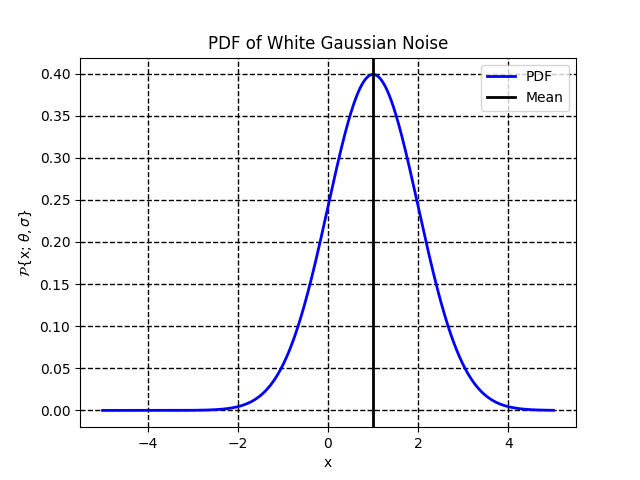
\includegraphics[width=0.5\textwidth]{assets/wgn.png}
    \end{center}
    \label{fig:wgn}
\end{figure}

There are two general classes of estimators:
\begin{enumerate} 
    \item \textbf{Classical Estimators:} The Parameters to be estimated are Deterministic as shown in equation \ref{eq:classical_e}.
    \begin{equation} \label{eq:classical_e}
        \hat{\theta} = g(x) \; \text{where} \; \mathcal{P}\left\{x; \theta\right\} \; \text{is the PDF of x}
    \end{equation}
    \item \textbf{Bayesian Estimators:} The Parameters to be estimated are Random Variables and their moments are to be estimated. These are described in equation \ref{eq:bayesian_e}
    \begin{equation} \label{eq:bayesian_e}
        \hat{\theta} = g(x) \; \text{where} \; \mathcal{P}\left\{x|\theta\right\} \mathcal{P}\left\{\theta\right\}\; \text{is the PDF of x}
    \end{equation}
\end{enumerate}

An estimator is just a transform of one random variable to another. An estimator takes realization of a random variable and gives the best guess of the parameter that it was designed to estimate. An estimator boils down to a random variable which has a mean equal the parameter in question and with as low a variance as possible. This needs to be established using Monte Carlo simulations.